\subsubsection{Plataforma Hardware Summit XL}

La capa robótica está constituida por la plataforma móvil Summit XL, desarrollada por Robotnik Automation, que actúa como elemento físico principal del sistema experimental. Se trata de una base móvil de propósito general orientada a aplicaciones de investigación y vigilancia en entornos interiores y exteriores. Esta capa integra los subsistemas mecánicos, de control, computación embarcada y sensórica necesarios para la operación tanto teleoperada como autónoma. En la Fig.~\ref{fig:summit} se muestran diferentes vistas de la plataforma.

\begin{figure}[H]
    \centering
    \begin{subfigure}{0.25\linewidth}
        \centering
        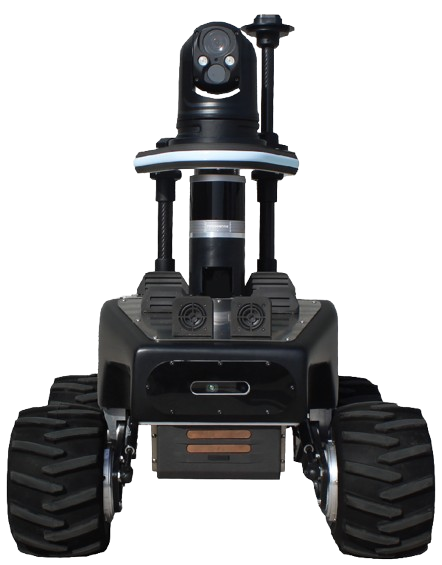
\includegraphics[width=\linewidth]{figures/robotnik_rb_summit_front.png}
        \caption{Vista frontal}
        \label{fig:summit_a}
    \end{subfigure}
    \hfill
    \begin{subfigure}{0.25\linewidth}
        \centering
        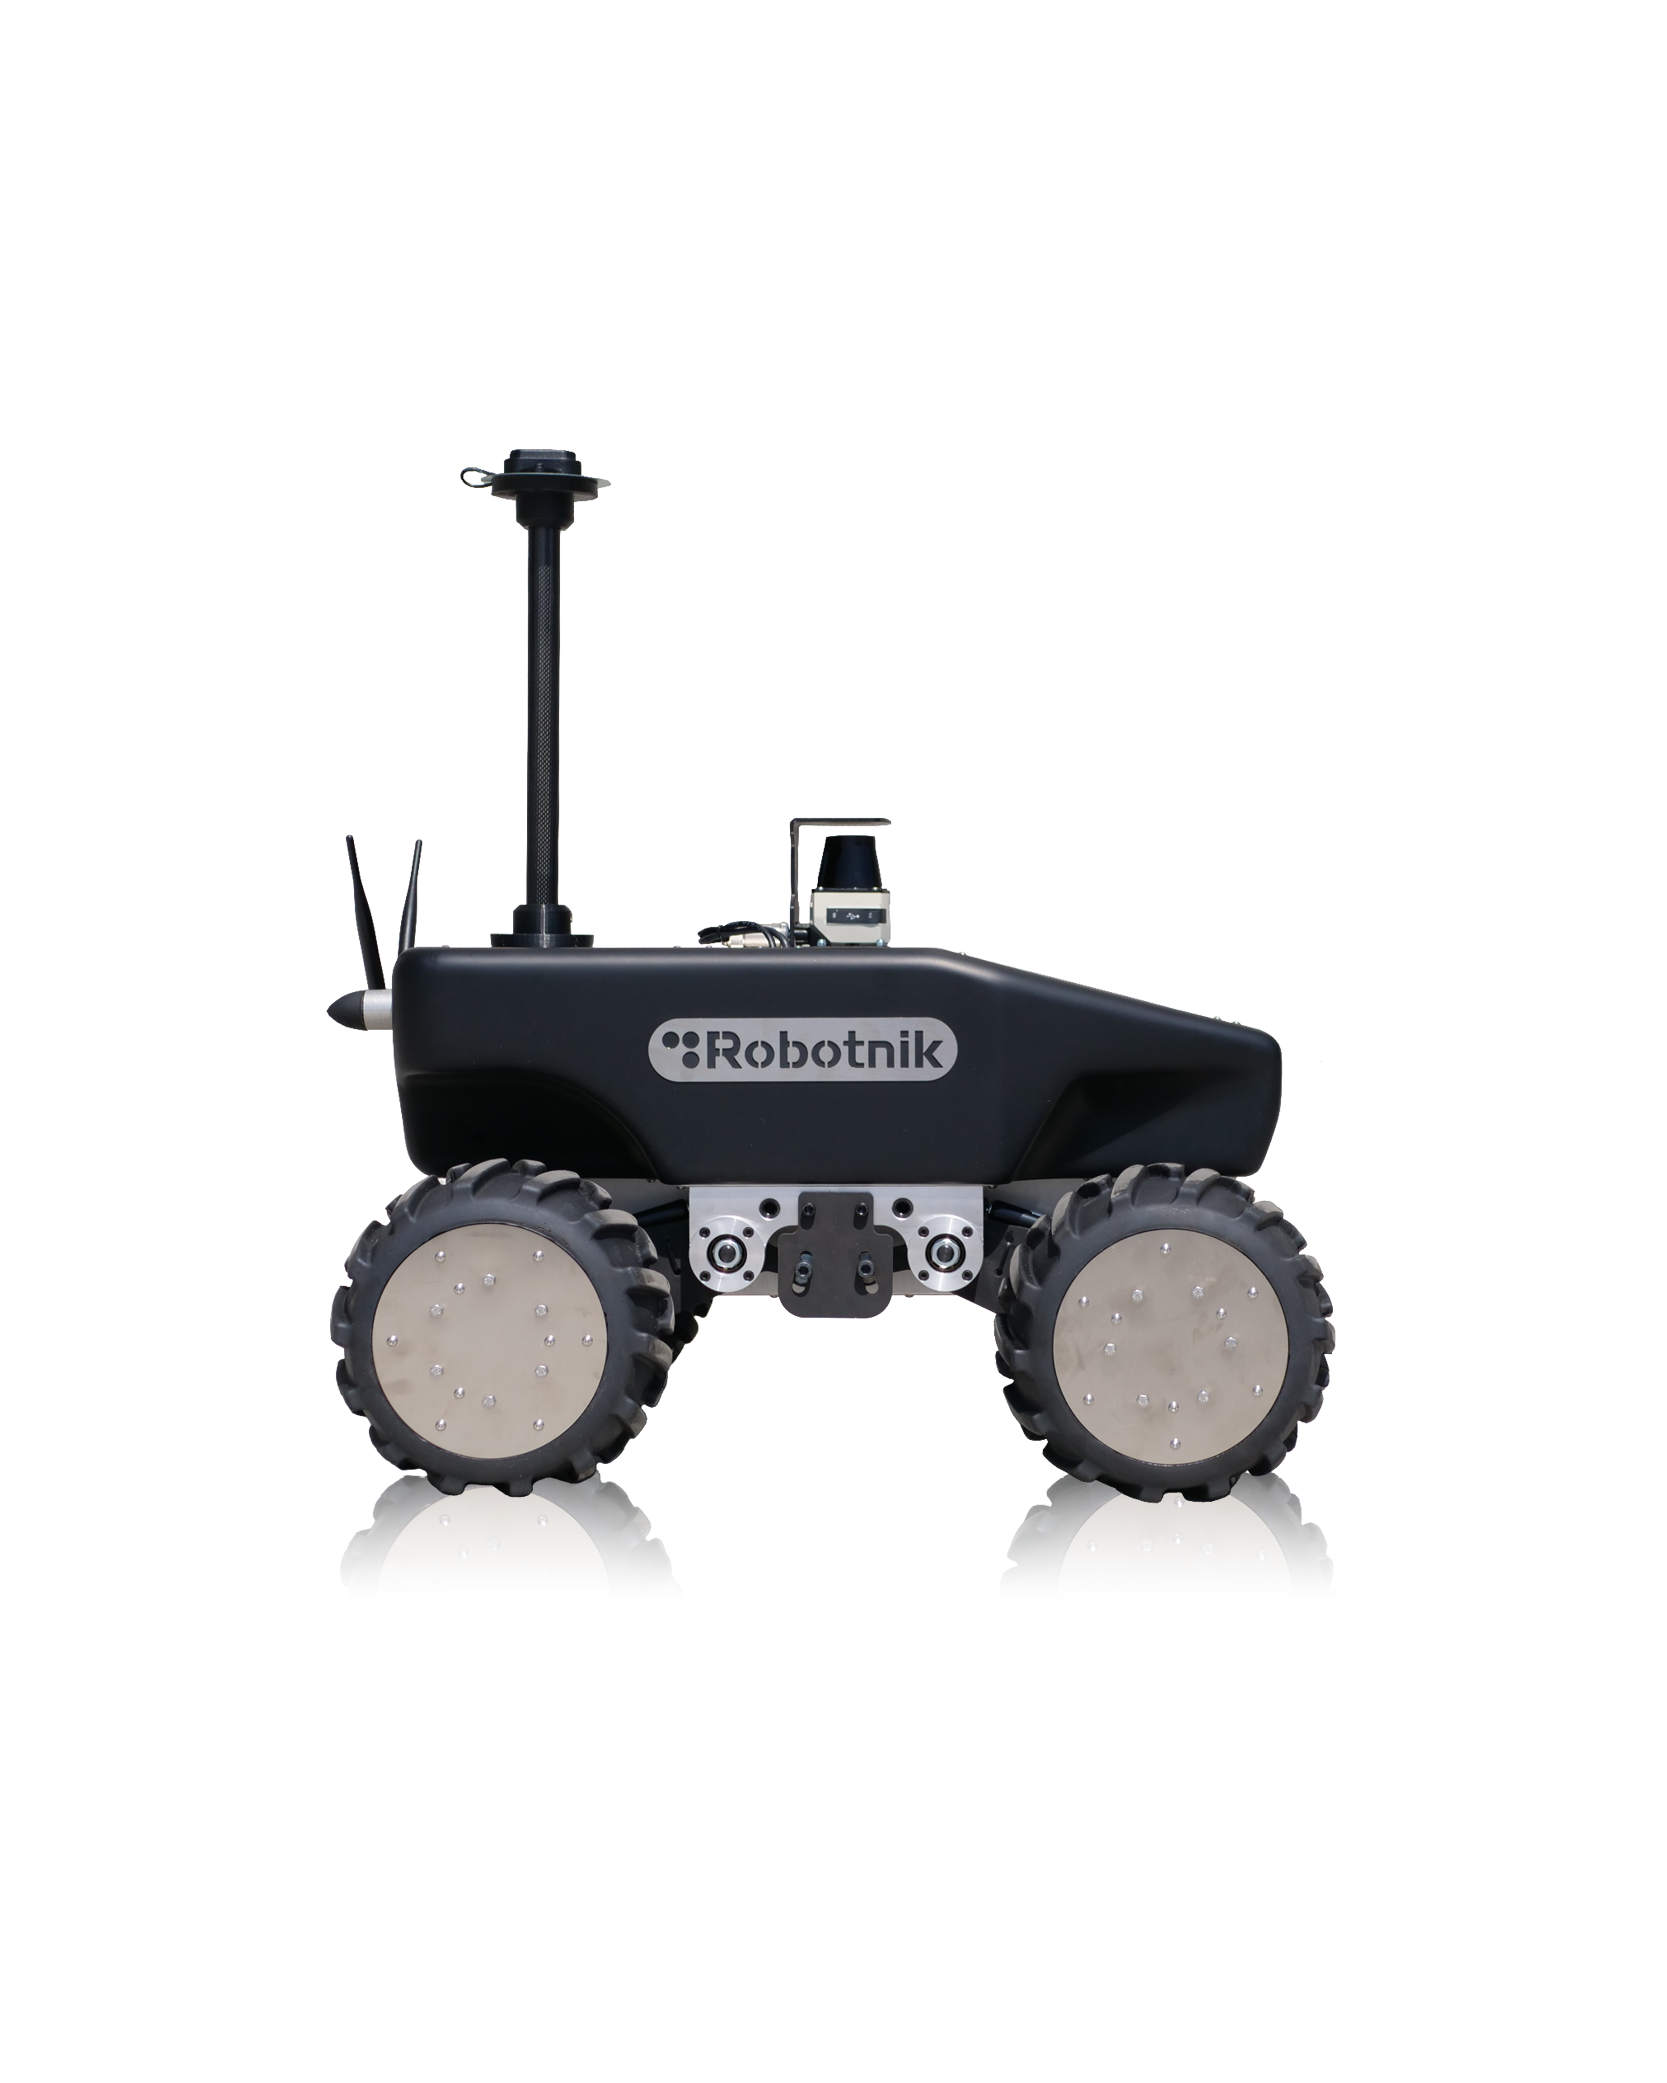
\includegraphics[width=\linewidth]{figures/robotnik_rb_summit_lateral.png}
        \caption{Vista lateral}
        \label{fig:summit_b}
    \end{subfigure}
    \hfill
    \begin{subfigure}{0.25\linewidth}
        \centering
        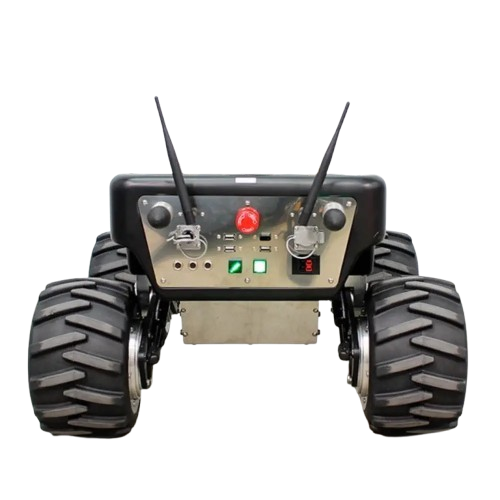
\includegraphics[width=\linewidth]{figures/robotnik_rb_summit_front_back.png}
        \caption{Vista trasera}
        \label{fig:summit_c}
    \end{subfigure}
    \caption{Plataforma Summit XL}
    \label{fig:summit}
\end{figure}

El Summit XL dispone de cuatro ruedas motrices con tracción diferencial tipo \textit{skid-steering}, donde el giro se produce mediante deslizamiento controlado provocado por la diferencia de velocidad entre los laterales derecho e izquierdo. Tiene una elevada capacidad de tracción y robustez mecánica.

El sistema de tracción está compuesto por:
\begin{itemize}
    \item Cuatro servomotores \textit{brushless} de 500 W.
    \item Encoders integrados para realimentación de velocidad y posición.
    \item Controladores de motor interconectados mediante bus \gls{can}.
\end{itemize}

La plataforma alcanza una velocidad máxima de 3 m/s y puede superar pendientes de hasta el 80\%, lo que la hace adecuada para escenarios exigentes.

Las principales especificaciones físicas del robot se recogen en la Tabla~\ref{tab:especificaciones_summit_xl}.

\begin{table}[H]
    \centering
    \begin{tabular}{|l|c|}
        \hline
        Dimensiones & 720 × 614 × 416 mm \\ \hline
        Peso & 65 kg \\ \hline
        Capacidad de carga & 50 kg \\ \hline
        Protección & IP50 \\ \hline
        Rango de temperatura & -10 °C a +45 °C \\ \hline
    \end{tabular}
    \caption{Especificaciones técnicas principales}
    \label{tab:especificaciones_summit_xl}
\end{table}

El sistema de alimentación se basa en una batería LiFePO$_4$ de 15 Ah a 48 V, proporcionando una autonomía de hasta 10 horas en función del perfil de operación.

La plataforma integra un PC industrial embarcado basado en Linux que actúa como unidad central de procesamiento, coordinando el control de actuadores y la adquisición de datos sensoriales. La arquitectura \textit{software} se basa en \gls{ros1}. La arquitectura basada en nodos permite desacoplar los módulos de percepción, localización, planificación y control, habilitando su ejecución local o su externalización hacia la infraestructura Edge a través de la red \gls{5g} privada.


La comunicación entre el ordenador embarcado y los drivers de motor se realiza a través del bus \gls{can}, lo que garantiza comunicación determinista y baja latencia en el control de actuadores.

En términos de conectividad, la plataforma dispone de:
\begin{itemize}
    \item WiFi 802.11n (WiFi-4).
    \item Conectividad interna: USB, RS232 y GPIO.
    \item Conectividad externa: USB, RJ45 y 12 VDC.
\end{itemize}

Estas interfaces permiten la integración directa con la infraestructura de red \gls{5g} privada, descrita en la sección \ref{sec:capa_de_red_5g_privada}, facilitando la transmisión de datos de percepción y control hacia nodos \textit{Edge} distribuidos.

La plataforma admite la integración de distintos sensores en función del caso de uso. En la configuración empleada en este trabajo se consideran:
\begin{itemize}
    \item Unidad de medición inercial (IMU).
    \item Cámara \gls{ptz} para transmisión de vídeo en tiempo real.
    \item Sensor \gls{lidar} para percepción del entorno.
\end{itemize}

De este modo, la plataforma robótica constituye el origen de los flujos de datos de percepción y control que serán procesados localmente o externalizados según la estrategia de \textit{offloading} definida en la arquitectura global del sistema, integrando la capa física con la infraestructura de computación distribuida descrita en capítulos anteriores.